\documentclass[twocolumn]{IEEEtran}
\renewcommand\IEEEkeywordsname{Palabras Claves}
\usepackage{cite}
\usepackage[utf8]{inputenc}
\usepackage{graphicx}
\usepackage{graphics}
\usepackage[spanish]{babel}
\usepackage[cmex10]{amsmath}
\interdisplaylinepenalty=2500
\usepackage{pgfplots}
%\usepackage{algorithmic}
\usepackage{array}
\usepackage{mdwmath}
\usepackage{mdwtab}
%\usepackage{eqparbox}
\usepackage[tight,footnotesize]{subfigure}

\begin{document}
%% Se puede usar \\ para darle el formato deseado
\title{Midgard}
%%%%%%%%%%%%%%%%%%%%%%%%%%%%%%%%%%%%%%%%%%%%%%%%%%%%%%%%%%%%%%%%%%%%%%%%%%%%%%%%%%%%%%%%%%%%%%%%%%%%%%%%%%%%%%%%%%%
% una imagen

%\begin{figure}[h!]
%\centering
%\includegraphics[width=\columnwidth]{NOMBRE.png}
%\caption{DESCRIPtION}
% \label{fig:crossover}
%\end{figure}
%\ref{fig:crossover}   
%THIS is for making a citation of the image otuside the declaration


%hacer una tabla:

%\begin{table}[h!]
%\centering
%\caption{Teorema de Thévenin y Norton}
%\begin{tabular}{c c c c c}
%\hline
%{\bf Rcar(Kohm)}&{\bf Corri.teór$[mA]$}&{\bf Corri.exp$[mA]$}&{\bf Pot.teó$[mW]$} &{\bf Pot.exp$[mW]$} \\ \hline
%{$0,4579$}&{$2,50$}&{$2,20$}&{$2,86$}&{$2,22$}\\
%{$0,9140$}&{$2,09$}&{$2,03$}&{$3,99$}&{$3,77$}\\
%{$1,376$}&{$1,80$}&{$1,82$}&{$4,46$}&{$4,56$}\\
%{$1,837$}&{$1,56$}&{$1,42$}&{$4,47$}&{$3,70$}\\
%{$2,280$}&{$1,39$}&{$1,45$}&{$4,40$}&{$4,80$}\\
%{$2,746$}&{$1,25$}&{$1,21$}&{$4,29$}&{$4,02$}
%\end{tabular}
%\end{table}


%hacer una grafica:

%\begin{tikzpicture}
%\begin{axis}[
%    title={Gráfico P Teórica vs R$_L$},
%    ylabel={Potencia [mW]},
%    xlabel={Resistencis [ohmios]},
%    xmin=0, xmax=3,
%    ymin=0, ymax=5.1,
%    xtick={0, 0.5, 1, 1.5, 2, 3},
%    ytick={0, 1, 2, 3, 4, 5},
%    legend pos=north west,
%    ymajorgrids=true,
%    grid style=dashed,
%]
 
%\addplot[
%    color=blue,
%    mark=square,
%    ]
%    coordinates {
%    (0.4579, 2.86)(0.9140, 3.99)(1.376, 4.46)(1.837, 4.47)(2.280, 4.40)(2.746,4.29)};
%\end{axis}
%\end{tikzpicture}


%% Los autores y su respectiva afiliacion, se usa ~ para evitar que corte la linea
\author{Abraham Arias\\
        e-mail:ipseabraham@gmail.com\\
        Fabian Solano\\
        e-mail:fasm2296@gmail.com\\
        Lenin Torres\\
        e-mail:ttvleninj@gmail.com\\
        Mauricio Montero Jiménez\\
        e-mail:maumonteroj@gmail.com\\
}

\makeatletter
\def\markboth#1#2{\def\leftmark{\@IEEEcompsoconly{\sffamily}\MakeUppercase{\protect#1}}%
\def\rightmark{\@IEEEcompsoconly{\sffamily}\MakeUppercase{\protect#2}}}

\maketitle


\begin{abstract}
%% menor de 3 parrafos, contiene teoria, actividades y conclusion.
%\section{Abstract}

Machines can't improvise well, because you can't program a fear of death (Interstellar 2014), our work is to challenge this affirmation, by the use of genetic algorithms in c++, which is the nearest approach of all the members of the group have been to any kind of artificial intelligence.\\ 
This document covers from the basic steps in the creation of a genetic algorithm, to any analysis to accomplish improvements by intense testing of our software. In addition we also explain how we handle hardware to create random numbers\cite{21}.\\
This genetic algorithm will represent villages including as many logical details according to reality (mutation, randomness, among others) and fantasy as possible. This towns are formed by many individuals with particular behaviors such as monogamy, life time, superstition, reproduction and many more, to ensure that their genetic information survives.\cite{20} \cite{14} \cite{15}\\

\end{abstract}



\section{Introduction}
Our code will represent concurrently each time a given number of different civilizations, they have a unique goal reproduce as many times as possible, the more suitable they are, more changes to reproduce. Also Combining genetic information, until they reach at top line, where no more changes occur or we decide to end the process. The fittest have more chances to reproduce that is what represents the natural selection process that we will be testing. At the end, the final solution will be tested against the gods, in a fight, and that defines if we get a solution by our genetic code.


\section{User Manual}



\section{Libraries and functions}

	\begin{enumerate}
    
    	\item Standard Library in C ++ \\
        C is a general-purpose, procedural, imperative computer programming 
        language developed in 1972 by Dennis M. Ritchie at the Bell Telephone 
        Laboratories to develop the Unix operating system. The C Standard 
        Library is a set of C built-in functions, constants and header files  
        like <stdio.h>, <stdlib.h<math.h>,etc. This library will work as a
        reference manual for C programmers.\cite{6}\cite{18} \\
    
        \item stdint.h\\
        This header was introduced in C99. to allow programmers to create integer 
        types more portable. This types have previously defined their sizes.\\ It is 
        possible to classify them into two kinds, the signed and unsigned, this 
        classification is visible from their type name. The range of widths are from 
        eight bits to the maximum size of a integer.\cite{8}\\
    
        \item Libserial\\
        It provides a collection of C++ classes that allow one to serial ports on 
        POSIX systems like standard C++ iostream objects. With this library we 
        successfully achieve:
        \begin{enumerate}
        \item Simplified serial port programming in C++ under POSIX operating systems\
        \item Support for USB-serial converters.\
        \item Access serial ports from scripting languages such as 									
        PHP, Python, Perl, Ruby, and Java (coming soon in version 0.6.0).\
		\end{enumerate}
            
         \item Tinyxml 1 \\
         Is a simple, small, C++ XML parser that can be easily integrating into other programs. In 
         brief, TinyXML parses an XML document, and builds from that a Document Object Model (DOM) that 
         can be read, modified, and saved.\cite{16}\\
         
         \item POSIX library.S unistd.h - standard symbolic constants and types.\\
         The <unistd.h> header defines miscellaneous symbolic constants and types, and declares 
         miscellaneous functions.\\
            
         \item Rand \\
         Returns a pseudo-random integral number in the range between 0 and max value. This number is 
         generated by an algorithm that returns a sequence of apparently non-related numbers each time 
         it is called. This algorithm uses a seed to generate the series, which should be initialized 
         to some distinctive value using function srand.\cite{17}\\
            
         \item fstream \\
         Input/output stream class to operate on files. Objects of this class maintain a filebuf object 
         as their internal stream buffer, which performs input/output operations on the file they are 
         associated with (if any). File streams are associated with files either on construction, or by 
         calling member open.\\
         
         \item OpenCv
         OpenCV is released under a BSD license and hence it’s free for both academic and commercial 
         use. It has C++, C, Python and Java interfaces and supports Windows, Linux, Mac OS, iOS and 
         Android. OpenCV was designed for computational efficiency and with a strong focus on real-time 
         applications. Written in optimized C/C++, the library can take advantage of multi-core 
         processing. Enabled with OpenCL, it can take advantage of the hardware acceleration of the 
         underlying heterogeneous compute platform. Adopted all around the world, OpenCV has more than 
         47 thousand people of user community and estimated number of downloads exceeding 9 million. 
         Usage ranges from interactive art, to mines inspection, stitching maps on the web or through 
         advanced robotics.

	\end{enumerate}



\section{Data structures}

	\begin{enumerate}
		\item Generic Circular Linked List\\
        
        Is the same definition of a linked list, but now it is double connected and also the 
        tail contains a pointer to the head, this is its particular characteristic.
     	   \begin{figure}[h!]
				\centering
				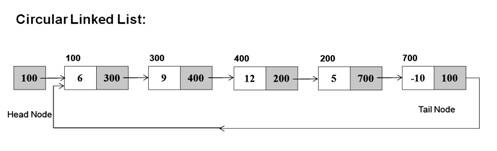
\includegraphics[width=\columnwidth]{src/circularLinkedList.jpg}
				\caption{Circular Linked List}
			\end{figure}\\
		Other particular characteristic is that this data structure it is able to handle any 
        kind of objects inside, thanks to the use of templates.\\
        
        \item Generic Array\\
        The PyArray class, is an implementation we had to do for using the matrix correctly, because we were not able to return a \textit{int matrix[30][30]} in an specific method. The best option was to make our own array class.\\ 
        Even though, the PyArray class is based on Python's array, it is not even a real Array, it is just a list with lists.\\ 
        In this specific problem, the time required to access the data was not important, but the way to access in a comfortable way was much more important.\\

\begin{figure}[h!]
				\centering
				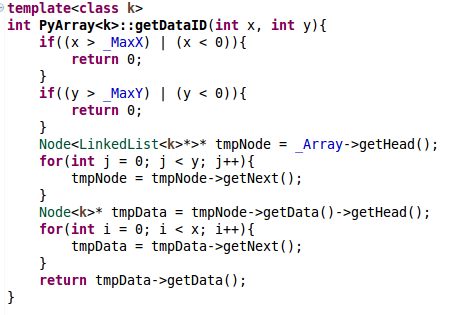
\includegraphics[width=\columnwidth]{src/getDataID.png}
				\caption{getDataID Method}
			\end{figure}
            
    	\item Bit Vector\\
        The bit vector is a class that we each bit position can be accessed individually which allows us to control a value at the bit level \cite{2}. This class is particularized to use logical operators (OR, AND, or other) against the value or bit string that will be used to get a bit of value in any position or place a bit of value in any position.\\ 
        In this specific problem, a human genome where each chromosome is a series of bits are simulated, where the bit vector allows us to change or get a bit of each chromosome.The following algorithms are used to implement the bit vector.\\ 
        \begin{figure}[h!]
        \centering
        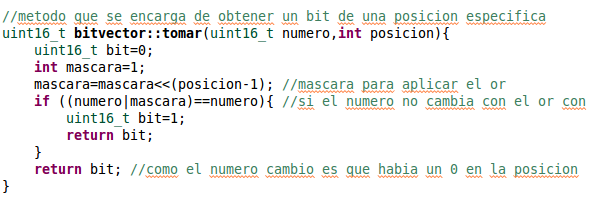
\includegraphics[width=\columnwidth]{src/bitvectortomar.png}
        \caption{Bitvector Method}
        \end{figure}
        
        \begin{figure}[h!]
        \centering
        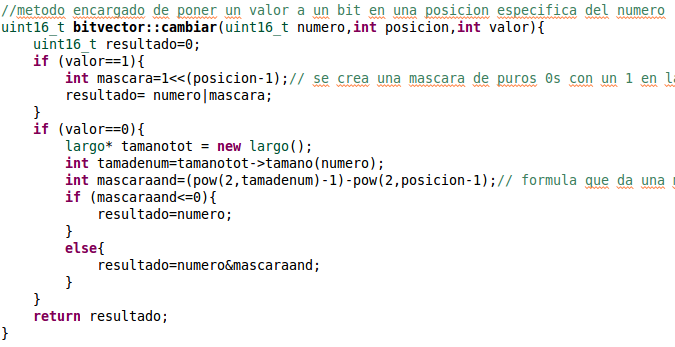
\includegraphics[width=\columnwidth]{src/bitvectorponer.png}
        \caption{Bitvector Method}
        \end{figure}
        The images show the method to take and put a bit,long way in putting a method that returns the length of a binary number. In the method take is used a mask of 0s and in the method put is uses a mask of 0s and 1s.

\end{enumerate}

    
\section{Circuit Design}
During the first days of development we analyze the importance of develop the circuit, so we would be able to test the algorithm using our own number generator. Around the web, there is not a lot of documentation about and specific circuit for do so.

\begin{enumerate} 
	\item Random Number Generator by IC 4017 and 4011\\
    
    After some research we realize that many people use the 4017 IC to generate random numbers so we try to use it to our project. But before doing it physically we prefer to run it on a circuit simulator program such as MultiSim, which allowed us to identify if the circuit will actually work or not. After some tests in the program, the circuit was not doing its full functionality as expected.
    \begin{figure}[h!]
	\centering
	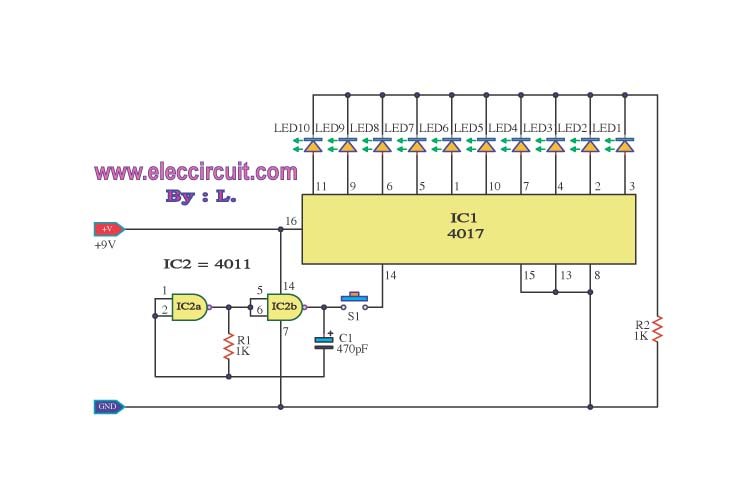
\includegraphics[width=\columnwidth]{src/Rand_V1.jpg}
	\caption{Circuit Design A}
	\end{figure}\\
    
    Using this circuit the numbers that were generated were not random. It seemed just to be a simple number counter. Even, most people said it should work. So this design was discarded.\\
    
    \item The "First Cut" Zener Noise Design\\
    
    The first approach using this new method, was to produce zener noise, which has been used many times. But in published circuits, this always had the problem that higher voltages were required than we might prefer. The voltage problem is attacked here by using an IC "zener" device, which has a low zener voltage. Also, some past designs have used digital circuits in so-called linear modes, again to support low-voltage operation. The intent here is to pretty much use the components the way they were intended to be used. Although we thought this should have work, it did not work properly. And the main reason was we did not use the required zener diode, but try to emulate it using two different zener diodes.
    
    \begin{figure}[h!]
	\centering
	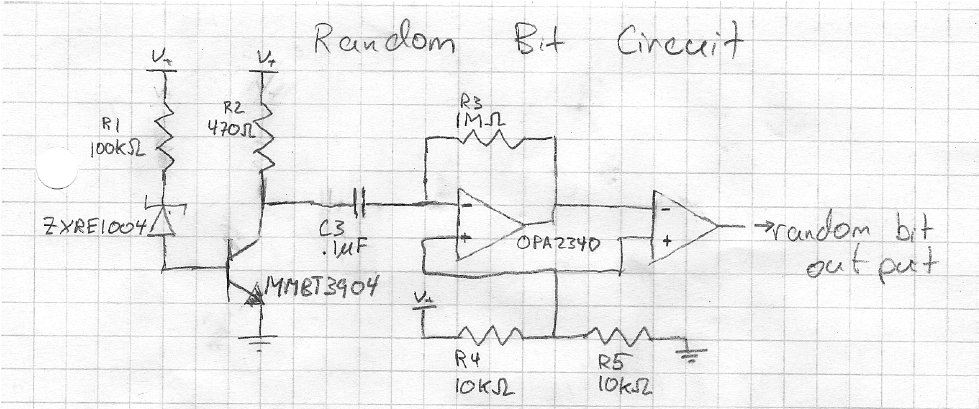
\includegraphics[width=\columnwidth]{src/Rand_V2.jpg}
	\caption{Circuit Design B}
	\end{figure}
    
    \item Amplified Noise Generator\\
    
    Because of the unsatisfactory results with previous circuits, we decided to change the objective a little bit from the original. We did some research on how to generate a single bit that was truly random. Based on the basic computer principle, Why do we use binary in computers? Because of its simplicity and because its easier to retrieve lost data, in our case its easier to generate a single random bit, instead of generating the whole number at once.
    
    \begin{figure}[h!]
	\centering
	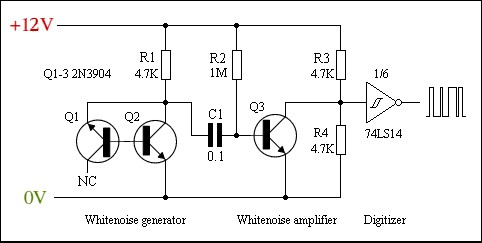
\includegraphics[width=\columnwidth]{src/Rand_V3.jpg}
	\caption{Circuit Design C}
	\end{figure}
    
    After some simple edits to the circuits such as the resistors values, and the adapter to the Arduino, we finally got a full functional circuit, that was able to generate truly random number based on noise in the proximity of the circuit. The following image, shows a graphic representation of the final circuit.
    \begin{figure}[h!]
	\centering
	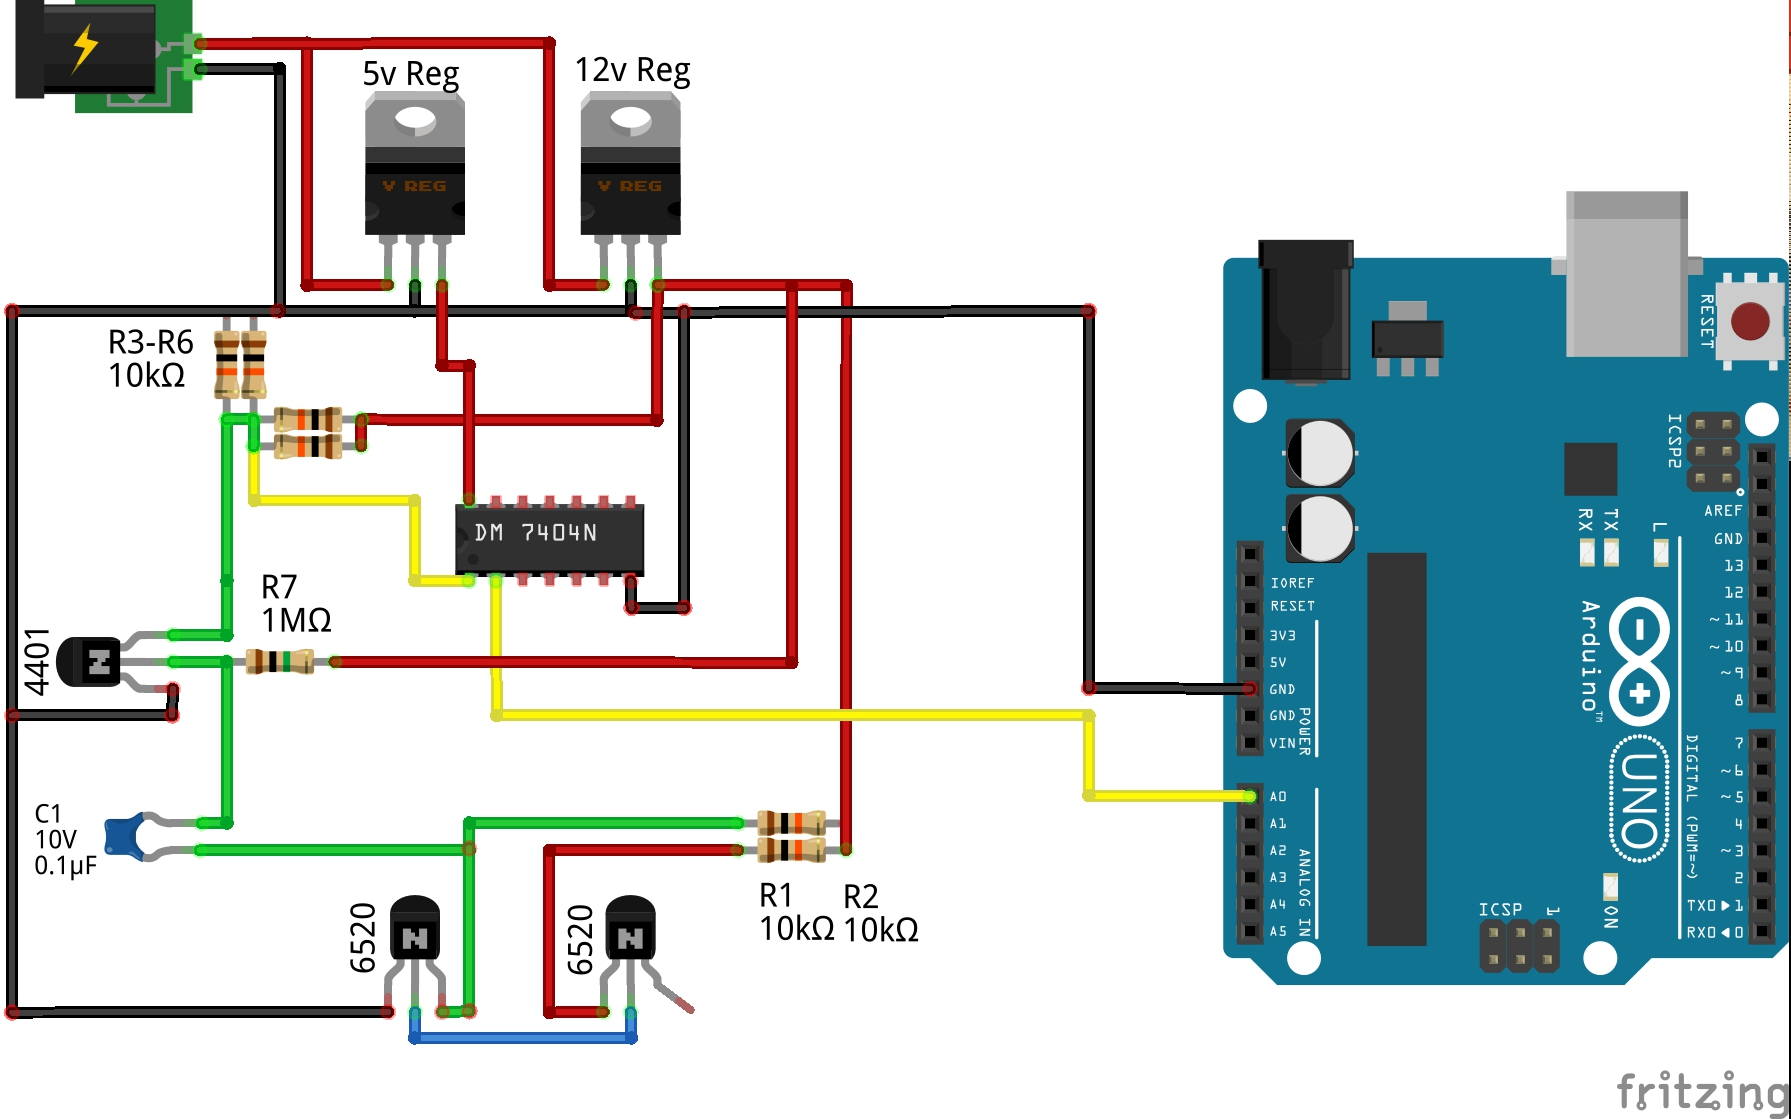
\includegraphics[width=\columnwidth]{src/Rand_Final.jpg}
	\caption{Circuit Final Design}
	\end{figure}
    
    To generate the number, we ask the circuit for a determined number of bits, if we want a small random number we should ask just for 5 bits, which gives us a max decimal number of 31. For example we ask the circuit for 5 random bits, and give us a random decimal number. The circuits returns 1,0,1,0,1. This data is stored in array, which later will be used to created the decimal number. We navigate through the array to start converting from binary to decimal which finally will give us 21 as the random number generated. With this method we can get as much random numbers as we want, and also specified the max number required, by giving the max bits to be generated as the main input. The following figure, shows the real circuit, as we finally finished building it.\\ An important detail to highlight is that when moving from breadboard to PCB, is really important to build the circuit using the diagram and make sure each connection is correct, because many times, a lot of time is wasted
    
    
    	
\end{enumerate}
   
   
   
   
\section{Algorithms}

Our genetic algorithm as any other follow a series of steps like any other, first we create the initial
population, and insert them into a loop\cite{GADarrelWitley}, where we calculate the fitness first, then select the fittest to reproduce, and finally select which ones stay and which others continuous alive.\cite{Electrophysiological} \cite{3} \\* 
    \begin{figure}[h!]
	\centering
	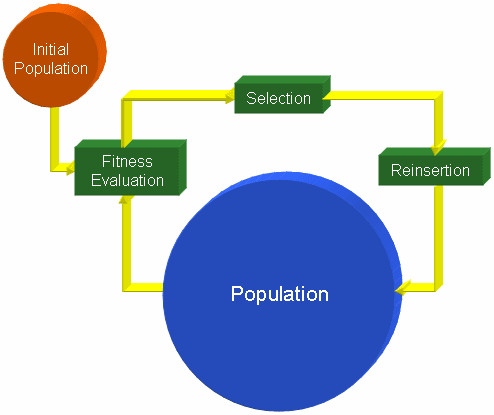
\includegraphics[width=\columnwidth]{src/GAalg.jpg}
	\caption{Steps of GA}
	\end{figure}
    
\begin{enumerate} 
	\item Fitness\\
    After just created the first generation, proceed with the function fitness, which is different 
    according to the individual's population, due to need to increase specific attributes in each 	
    population. But the main idea consist in divide one by one attribute of the individual between the 
    sum of all those attributes in the whole population, finally do this for the 8 characteristics and 
    put it together in number called fitness.\cite{9} \\
    
        \begin{figure}[h!]
        \centering
        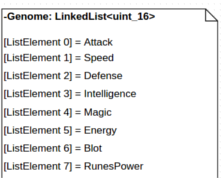
\includegraphics[width=\columnwidth]{src/cualidades.png}
		\caption{Genome Distribution}
		\end{figure}
        
        
    As each population have more value attributes, we need to calculate separately fitness for each  
    population, a more detail explanation is available in section Implemented methods.
        
        
    \item Crossover\\
    	Inspired in nature, we combine two possible solution, one from the mother and other from the 
        father to create a new offspring with similar attributes. \cite{4} \cite{5} \cite{7}
	    \begin{figure}[h!]
        \centering
        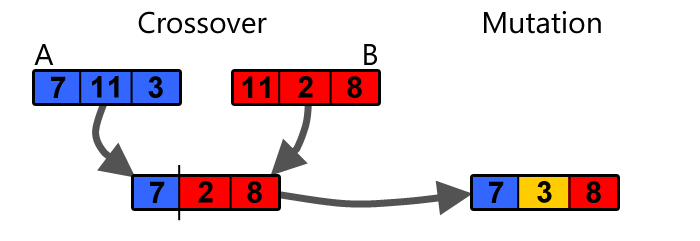
\includegraphics[width=\columnwidth]{src/crossover_mutation.png}
		\caption{Crossover and Mutation}
        \label{fig:crossover}
		\end{figure}
        We work with a simple crossover as the figure \ref{fig:crossover} shows, in which we take half 
        chromosome from the mother and the father and by a simple operations with masks and with 
        logical operators achieved the half and half combination. It is known that specific crossover
        help in particular cases, however in this project by the moment we keep this operation simple
        unless future testing proves deficiencies or needs of change in this area. 
        
        
    \item Mutation and Inversion
   	As in nature something unexpected events with genetic information causes disasters, other changes 
    may propitiate advantages to certain individuals, that is why we add a possibility of random changes
    in the genetic information, the proportion of that possibility is study in the section Results.\\
    
    
    \item Random Numbers.\\
    
    As explained before the random number generator circuit, only generates a single bit, a from that it starts to create a whole decimal number.\\
    The \textit{getNumber(int maxType} method, receives as a parameter the max number of bits to create the decimal number. It stores in an array the bits generated from the circuit, once all the bits are ready, it calls the \textit{randomNumber(int numArray[],int ind,int resultado,int maxType)} method, which starts moving through the array and with the general formula for converting from a base to another, it changes the binary digits on the array to a decimal number.\\
    The arduino sketch waits for a serial data to be available, this data will be the max number of bits to generate the number. This is very flexible, because from the C++ program, we can request any size of number, just by giving the max bits required.
    
    \begin{figure}[h!]
        \centering
        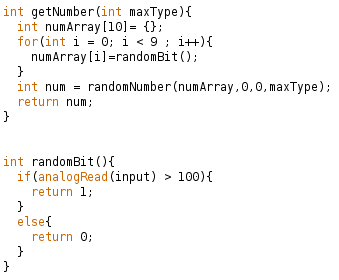
\includegraphics[width=\columnwidth]{src/ArduinoCode1.png}
		\caption{Arduino Code Part A}
        \label{fig:crossover}
		\end{figure}
        
        \begin{figure}[h!]
        \centering
        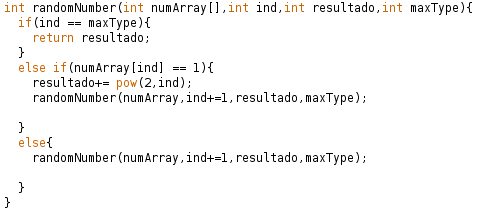
\includegraphics[width=\columnwidth]{src/ArduinoCode2.png}
		\caption{Arduino Code Part B}
        \label{fig:crossover}
		\end{figure}
        
\end{enumerate}



\section{Complexity Analysis}
This is a theoretical complexity analysis.
\subsection{First let's analyze the code in genetic} 
\begin{enumerate}

	\item Reproduction\\
    Iterates to reproduce a given number of entities. 
    First a crossover is realized. But there is not a direct function with this name, however the code that performs this is located in the reproduction class, in a method called reproduce. With the next complexity.  
    \begin{equation} O(n) \end{equation}
    The rest of the reproduction are assignations with constant complexity, so reproduction is defined recursively by the crossover.

	\item Fitness\\
	First we calculate the fitness, this calculus has a special modification, so the calculus of the fitness for any individual is constant. 
    \begin{equation} O(c) \end{equation}
    
    To achieve this, in the first generation we sum all the characteristics respectively of all the entities for each population. This part of the code has a higher complexity defined by the size of the first generation(n), that usually is very small. We call that method set Base in fitness.
    \begin{equation} O(n) \end{equation}\\
    
\end{enumerate}

\subsection{Methods in populations}
	The main methods along the process, are called by a method called Do a generation, which choose which ones reproduce, kill other, ages people as long the world decides.\\*
    So the complexity is defined by the most complex method coming up next.\\

\begin{enumerate}
	\item Get Random Number\\
    A variable for the hardware may be in two sates, false or true, in the first case a simple request of a random number provided by the c++ library is performed, otherwise the complexity is constant in our code that request a random number thought the serial communication to the Arduino. This is our bottleneck, that time consumed.\\
	\item Natural Selection\\
    	In this part we reproduce a random number of entities. First we need to assign more changes to the fittest individuals, and randomly choose two to reproduce.
        \begin{equation} O(n^2) \end{equation}\\
    \item Birthday for everybody\\
    A simple counter represents the age. Increases each loop.
    \begin{equation} O(n) \end{equation}\\
    
    \item Death\\
    When a entity gets too old, is very likely to die, that chances increases as it gets older.
    \begin{equation} O(n) \end{equation}\\ 
    
\end{enumerate}	








\section{Implemented methods} 
	\begin{enumerate}
    
    \item A* Algorithm\\
    
    In computer science, A* is a computer algorithm that is used in path finding and graph moving, the process of plotting an efficiently traversal path between multiple points, called nodes or blocks. This is mainly used because of its performance and accuracy, it enjoys widespread use. However, in practical travel-routing systems, it is generally outperformed by algorithms which can pre-process the graph to attain better performance.\\

Peter Hart, Nils Nilsson and Bertram Raphael of Stanford Research Institute first described the algorithm in 1968.It is an extension of Edsger Dijkstra's 1959 algorithm. A* achieves better time performance by using heuristics. Heuristic refers to the estimated movement cost to move from the given square on the grid to the final destination. The A* algorithm can be complicated at first, but by doing some research, reading about the implementation and by identify some examples around the web, understanding the main concept is really simple.\\

	\begin{enumerate}[Algorithm's Steps]
    
	\item Begin at the starting point A and add it to an “open list” of squares to be considered. The open list is kind of like a shopping list. Right now there is just one item on the list, but we will have more later. It contains squares that might fall along the path we want to take, but maybe not. Basically, this is a list of squares that need to be checked out.
    
    \item Look at all the reachable or walkable squares adjacent to the starting point, ignoring squares with walls, water, or other illegal terrain. Add them to the open list, too. For each of these squares, save point A as its “parent square”. This parent square stuff is important when we want to trace our path.
    
    \item Drop the starting square A from your open list, and add it to a “closed list”.
    
    \item Next, we choose one of the adjacent squares on the open list and more or less repeat the earlier process, as described below. But which square do we choose? The one with the lowest F cost.\\

Path Scoring\\

The key to determining which squares to use when figuring out the path is the following equation:\\

F = G + H \\

where\\

G = the movement cost to move from the starting point A to a given square on the grid, following the path generated to get there.\\ 
H = the estimated movement cost to move from that given square on the grid to the final destination, point B. This is often referred to as the heuristic, which can be a bit confusing. The reason why it is called that is because it is a guess. We really don’t know the actual distance until we find the path, because all sorts of things can be in the way (walls, water, etc). 

	\item To continue the search, we simply choose the lowest F score square from all those that are on the open list. We then do the following with the selected square. Drop it from the open list and add it to the closed list.
    
    \item Check all of the adjacent squares. Ignoring those that are on the closed list or unwalkable (terrain with walls, water, or other illegal terrain), add squares to the open list if they are not on the open list already. Make the selected square the “parent” of the new squares.
    
    \item If an adjacent square is already on the open list, check to see if this path to that square is a better one. In other words, check to see if the G score for that square is lower if we use the current square to get there. If not, don’t do anything. 
    On the other hand, if the G cost of the new path is lower, change the parent of the adjacent square to the selected square. Finally, recalculate both the F and G scores of that square.\\

	\end{enumerate}
    
    \begin{center}
    Bibliography
    \end{center}
	A* Path finding for Beginners. By Patrick Lester (Updated July 18, 2005). Retrieved May 4, 
    2015, from http://www.policyalmanac.org/games/aStarTutorial.htm\\*
    
    
    \item Map Editor\\
    A* Algorithm requires a lot of testing to verify its functionality, but manually modifying the matrix each time we want to test some changes to the algorithms design its kind of boring and complicated. To avoid manually modifying the matrix, a Map Editor was developed. This simple program was developed in Python 2.7 under Linux, the Python language was used to do so, because of its simplicity to develop the graphical user interface.\\
    Program functionality is really basic, it just identifies the current mouse coordinates inside the screen, and map it to a single matrix position, depending on the users path selection it changes the number in the matrix, the only walkable path is grass, which is represented by a "1", in the matrix. Other kinds of terrains are represented by numbers greater than "1". The following picture shows the Map Editor window, and a map loaded.
    \begin{figure}[h!]
        \centering
        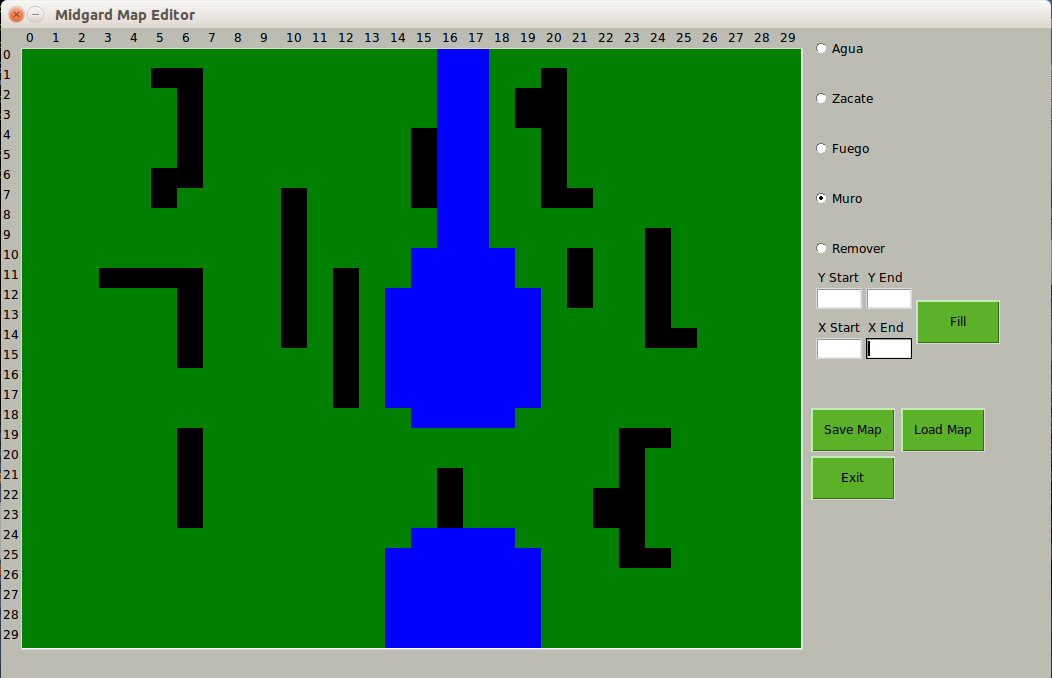
\includegraphics[width=\columnwidth]{src/MapEditor.png}
		\caption{Map Editor Graphical User Interface}
        \label{fig:crossover}
		\end{figure}
\end{enumerate}
    



\section{Techniques of algorithm's designs}

	As we have learned put some programmers to code by them selfs, so each make individual assumptions along  the project, and guessing about does not lead to success. That is why we decide to work as a whole team, approaching a least in some part some principles of several Techniques of algorithm's designs.
\begin{enumerate}
	\item Genetic Algorithm \\
    Our while project is base in this probabilistic techniques. The reason why we use genetic algorithms, is because on the first place we do not know in which environment our solution will be tested, that environment is defined by random goods created at the beginning, also with our villages. Otherwise a brute force solution may take too many attempts, even with some trimmings to the solutions, because it will have to start testing from scratch solution by solution. That's the reason why in this presented problem we took this approach. 


\end{enumerate}

\section{Results}

To ensure very representative data, we take 30 samples, and show an average, whenever possible.\\

\begin{enumerate}
\item {Genetic Algorithm Tests}\\

The following bar graphics represents tests made changing different parameters in the genetic algorithm. The x axis represent the current generation (each one represents one age to any individual), and the other axis represents the number of population. 
    
    \begin{figure}[h!]
    \centering
    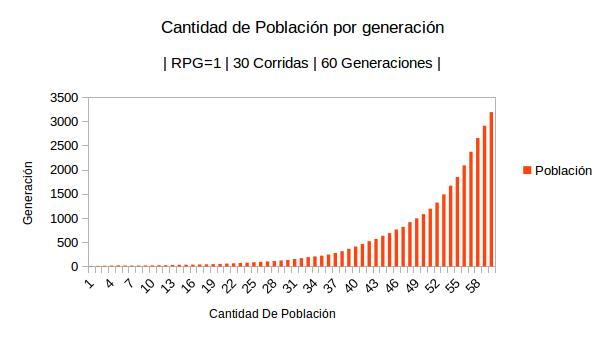
\includegraphics[width=\columnwidth]{src/rpg1.jpg}
	\caption{Graphic A}
    \label{fig:TESTRPG1}
    \end{figure}
    
In any given population we have a variable number of people per generation. As in reality we need two individuals to reproduce, in our case we do not care about having different sex in the reproduction. So at the moment to reproduce the generation, the maximum number of new borns will be the half of the population, just if by chance the random number generator indicates it, because to select the number of reproductions to realize in each generation, a random number is ordered. How ever if we always reproduce by a random number indicates, the growing of the population is to high, even when we start with 10 individuals, as the Figure \ref{fig:TESTRPG1} shows.\\


    \begin{figure}[h!]
    \centering
    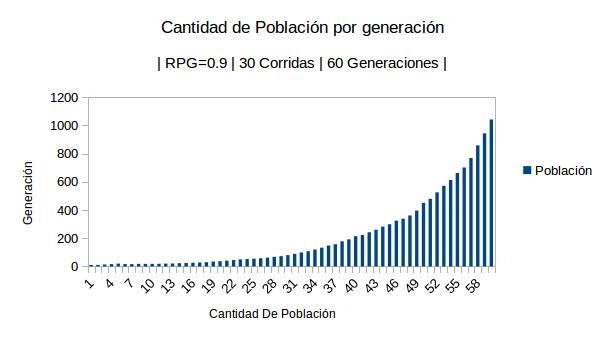
\includegraphics[width=\columnwidth]{src/rpg0_9.jpg}
	\caption{Graphic B}
    \label{fig:TESTRPG0.9}
    \end{figure}
    
When we decrease a variable called Number of generations per generation, what we do is to limit the maxim number of reproductions, by a simple restriction, the maximum number of generation is limited by a multiplication of the half of the population times the RPG variable(from 0 to 1), and that is the maximum possible number of reproductions given by the random.//   
    \begin{figure}[h!]
    \centering
    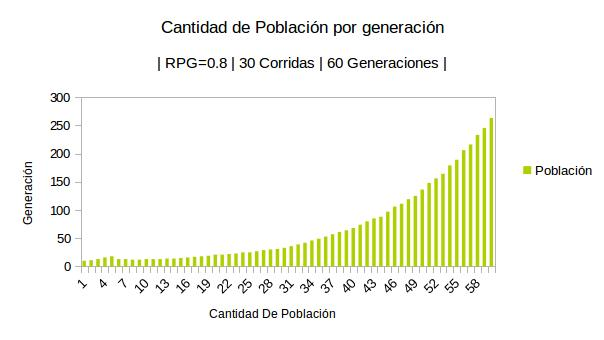
\includegraphics[width=\columnwidth]{src/rpg0_8.jpg}
	\caption{Graphic C}
    \label{fig:TESTRPG0.8}
    \end{figure}
    
    \begin{figure}[h!]
    \centering
    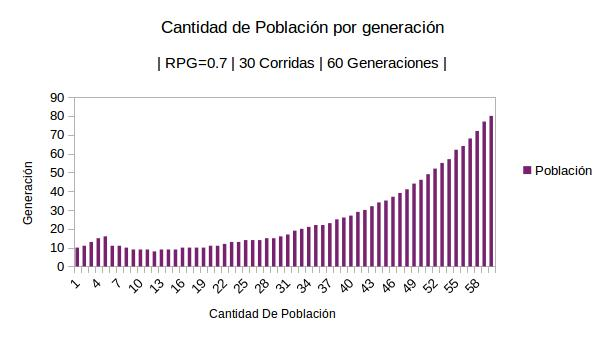
\includegraphics[width=\columnwidth]{src/rpg0_7.jpg}
	\caption{Graphic D}
    \label{fig:TESTRPG0.7}
    \end{figure}
    
    \begin{figure}[h!]
    \centering
    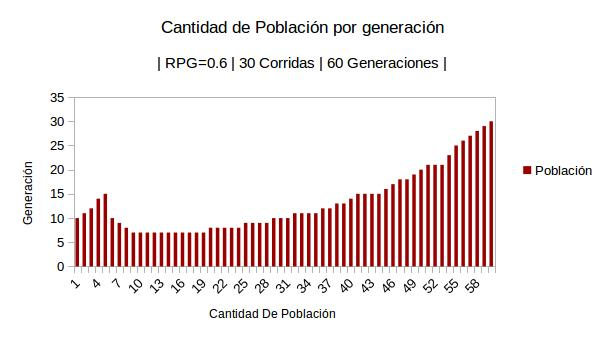
\includegraphics[width=\columnwidth]{src/rpg0_6.jpg}
	\caption{Graphic E}
    \label{fig:TESTRPG0.6}
    \end{figure}
    
    \begin{figure}[h!]
    \centering
    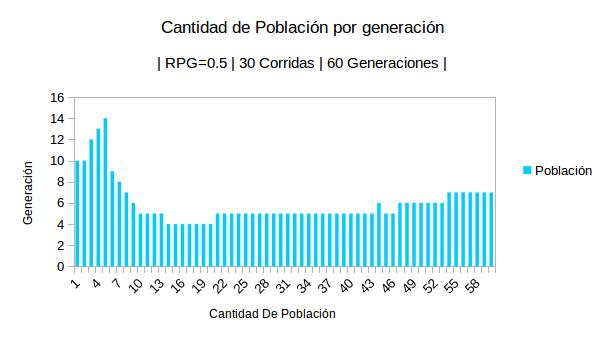
\includegraphics[width=\columnwidth]{src/rpg0_5.jpg}
	\caption{Graphic F}
    \label{fig:TESTRPG0.5}
    \end{figure}
    
    \begin{figure}[h!]
    \centering
    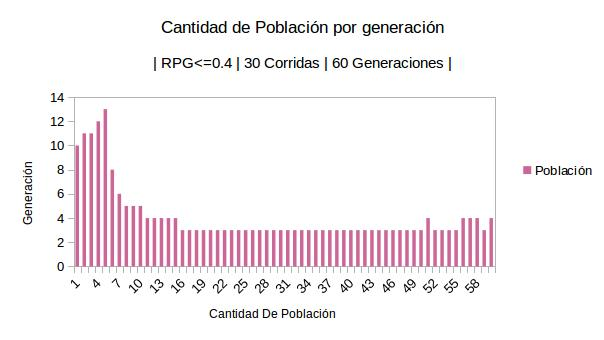
\includegraphics[width=\columnwidth]{src/rpg0_4.jpg}
	\caption{Graphic G}
    \label{fig:TESTRPG0.4}
    \end{figure}
    
From the figure \ref{fig:TESTRPG1} to the figure \ref{fig:TESTRPG0.6} the result of decreasing the RPG variable is very clear, the population growths more slowly each time. Even keeping in mind that when an entity reaches certain age, it is very likely to die, even more when it keeps getting older.//*  But in figure \ref{fig:TESTRPG0.5} and figure \ref{fig:TESTRPG0.4} the behavior does something odd, the number of population get static. Due to that unknown behavior, values lower than 0.6 are not useful. \\ 


	\item Fitness\\
    Through the fitness calculus show in the figure \ref{fig:fitness60g} and \ref{fig:strength60g} a simple crossover allow the grow in some features of our entities. However an inner analysis also shows also in the figure \ref{fig:fitness60g}, that the worst fitness is not getting any better, even it is dropping significantly. We decide to leave those guys existing with the same probabilities than the best ones just to maintain diversity in our genetic information.    
    
    \begin{figure}[h!]
    \centering
    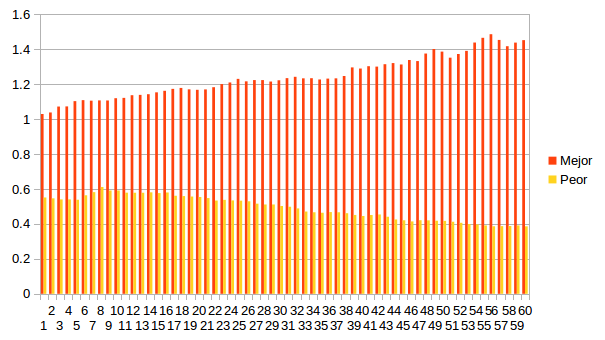
\includegraphics[width=\columnwidth]{src/bestcrossover.png}
	\caption{Fitness in 60 generations}
    \label{fig:fitness60g}
    \end{figure}
    
    \begin{figure}[h!]
    \centering
    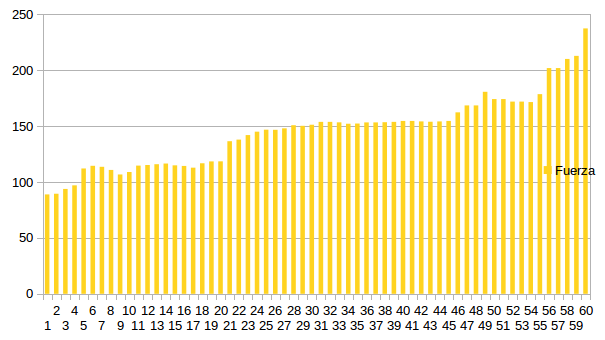
\includegraphics[width=\columnwidth]{src/crecimientodeFuerza.png}
	\caption{Growing of the strength}
    \label{fig:strength60g}
    \end{figure}
    
	\item Random Numbers.\\
    On the first place let's analyze the random number generator available in c++, so later we can compare.//
    
    \begin{figure}[h!]
    \centering
    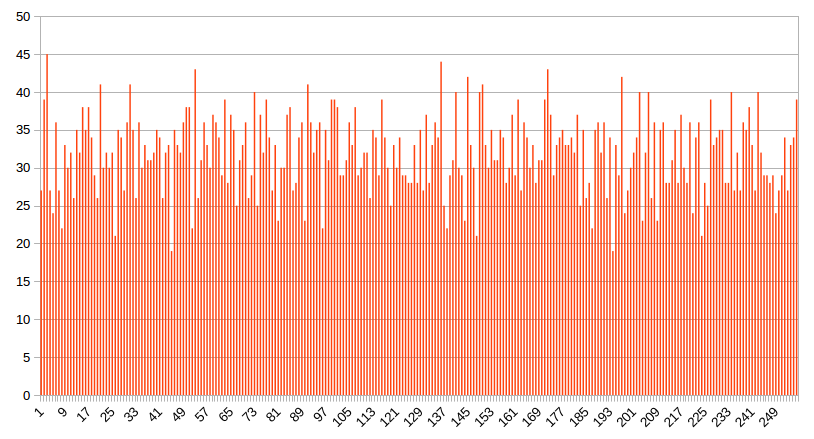
\includegraphics[width=\columnwidth]{src/RANDOMc++.png}
	\caption{256 random numbers from c++ library asked 8192 times}
    \label{fig:2n2048vc++}
    \end{figure}
    As we can see it is far from perfect, but patterns are not very clear, or at least in this graph.//*    
    Now we can present the results of our random number generator by hardware. As the circuit has been already explained, now let's just analyze the obtained data. \\*
    We create two automatized test, for six cases, on the first place we recompile many answers in a small range of two numbers, as the figures \ref{fig:2n2048v}, \ref{fig:2n4096v} and \ref{fig:2n8192v} shows.  \\* 
In these cases we can see a tendency to produce the cero more than the one in the three test.\\
	\begin{figure}[h!]
    \centering
    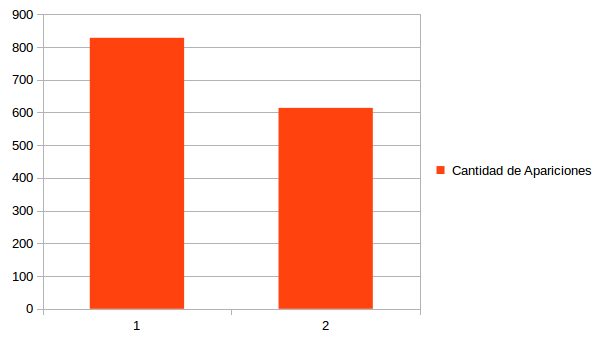
\includegraphics[width=\columnwidth]{src/2n2048v.png}
	\caption{Chart of 2 random numbers asked 2048 times}
    \label{fig:2n2048v}
    \end{figure}
    
    \begin{figure}[h!]
    \centering
    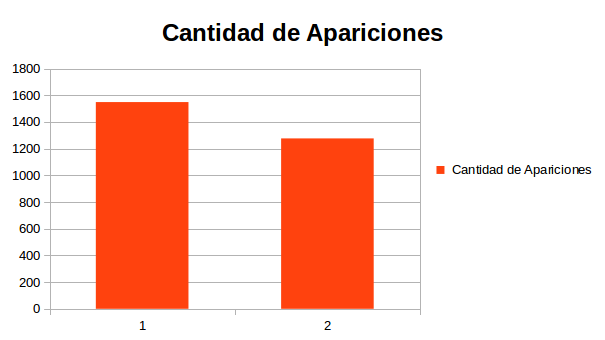
\includegraphics[width=\columnwidth]{src/2n4096v.png}
	\caption{Chart of 2 random numbers asked 4096 times}
    \label{fig:2n4096v}
    \end{figure}
    
    \begin{figure}[h!]
    \centering
    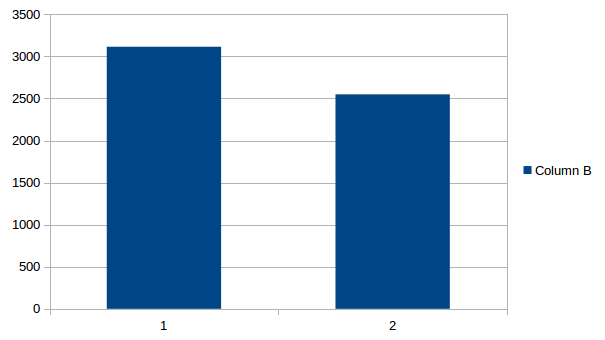
\includegraphics[width=\columnwidth]{src/2n8192v.png}
	\caption{Chart of 2 random numbers asked 8192 times}
    \label{fig:2n8192v}
    \end{figure}
    
To make more useful our circuit we also allow random ranges as bigger as we want. Also we test a bigger range of numbers, in  this case a range from 0 to 256, and ask as many times as we consider enough (8196 times). \\
As we can see in figures \ref{fig:256n2048v},\ref{fig:256n4096v} and \ref{fig:256n8192v} some kind of pattern is visible just by simple sight, exits gaps where some numbers have very low chance to be chosen. Also other particular behavior visible in these three graphs, where the higher possibilities of the numbers to be chosen are at the beginning. It does not have a linear distribution, as higher the number, apparently less chance to be taken.  

	\begin{figure}[h!]
    \centering
    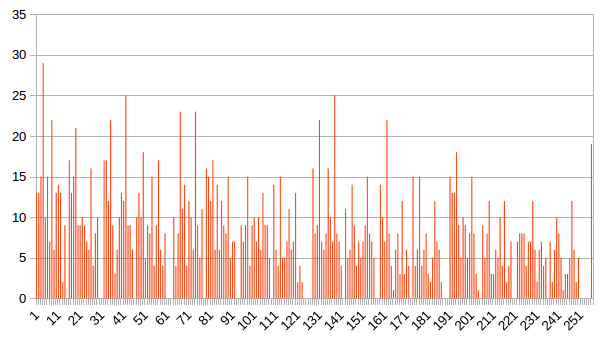
\includegraphics[width=\columnwidth]{src/256n2048v.png}
	\caption{Chart of 256 random numbers asked 2048 times}
    \label{fig:256n2048v}
    \end{figure}
    
    \begin{figure}[h!]
    \centering
    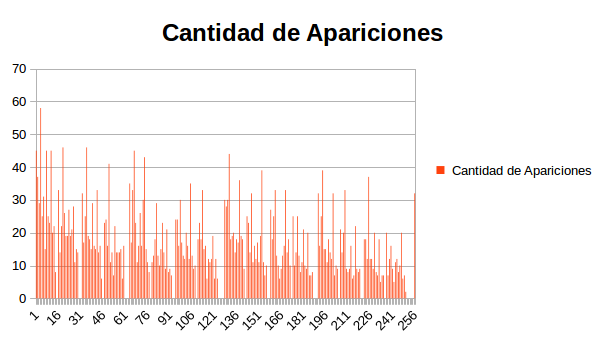
\includegraphics[width=\columnwidth]{src/256n4096v.png}
	\caption{Chart of 256 random numbers asked 4096 times}
    \label{fig:256n4096v}
    \end{figure}
    \begin{figure}[h!]
    \centering
    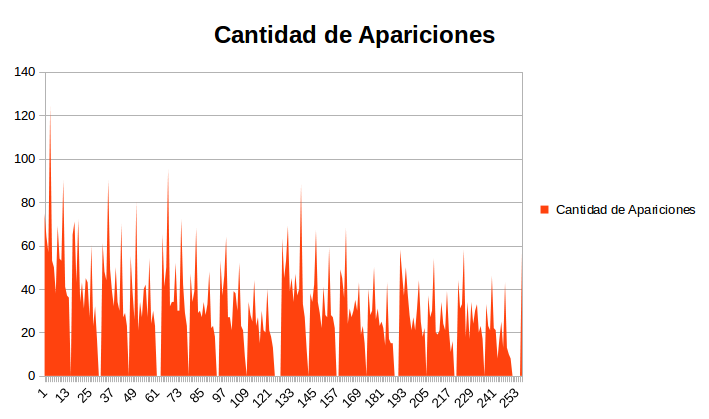
\includegraphics[width=\columnwidth]{src/256n8192v.png}
	\caption{Chart of 256 random numbers asked 8192 times}
    \label{fig:256n8192v}
    \end{figure}
    
	\end{enumerate}






\section{Design patterns}
	
    By trial and error many software developers suggest to follow some practices when developing software.
    \begin{enumerate}

	\item Singleton Pattern.
    This type of design pattern comes under creational pattern. In many situations we just want only and just one instance of an object. In our project we developed a class to handle all our constants, throughout the whole project it is not necessary to have two objects, to accomplish this this class contains a static method, which returns a instance of the only object created along the running program.    
    
	\end{enumerate}
    
\section{Activities by student}

Activities references \cite{LaTeXTemplates } \cite{10} \cite{11}\cite{latexjorg}

\begin{table}[h!]
\centering
\caption{Abraham's Activities}
\begin{tabular}{c c c}
\omit
{\bf Date}&{\bf Hours}&{\bf Activity}\\  \hline
{$05/16$}&{$1,5$}&{$Requirement analysis$}\\
{$05/17$}&{$1$}&{$SVN for code and documentation$}\\
{$05/20$}&{$4$}&{$Hierarchy of classes $}\\
{$05/26$}&{$4$}&{$crossover without bit Vector$}\\
{$05/00$}&{$2$}&{$Entities, vilalges classes $}\\
{$05/28$}&{$4$}&{$Fitness Function$}\\
{$05/29$}&{$5$}&{$We tried OpenCv$}\\
{$05/30$}&{$2$}&{$Population with our random$}\\
{$06/01$}&{$3$}&{$Graphs for random numbers$}\\
{$06/02$}&{$2$}&{$Death and selection functions$}\\
{$06/03$}&{$2$}&{$Documentation$}\\
{$06/08$}&{$2$}&{$deviation of the genetic information$}\\
{$06/20$}&{$2$}&{$Documentation$}\\
\end{tabular}
\end{table}


\begin{table}[h!]
\centering
\caption{Fabian's Activities}
\begin{tabular}{c c c}
\omit
{\bf Date}&{\bf Hours}&{\bf Activity}\\  \hline
{$05/22/15$}&{$3$}&{$Initial project setup meeting$}\\
{$05/23/15$}&{$3$}&{$Random number circuit research$}\\{$05/23/15$}&{$2$}&{$Setupo random number problem$}\\
{$05/24/15$}&{$3$}&{$New research for a random number circuit$}\\
{$05/24/15$}&{$2$}&{$Circuit emulation using MultiSim 12$}\\
{$05/24/15$}&{$3$}&{$Test the circuit on breadboard$}\\
{$05/24/15$}&{$2$}&{$Elaboration of the circuit on PCB$}\\
{$05/25/15$}&{$2$}&{$Check circuit usability$}\\
{$05/25/15$}&{$4$}&{$Basic classes for the simulation$}\\
{$05/25/15$}&{$1$}&{$TinyXML installation, Constatns Class$}\\
{$05/25/15$}&{$4$}&{$Genome,Entity classes and main logic$}\\
{$05/25/15$}&{$4$}&{$Random name obtainer for Entity class$}\\
{$05/25/15$}&{$2$}&{$Arduino and C++ communication$}\\
{$05/26/15$}&{$2$}&{$Changed the circuit power supply$}\\


\end{tabular}
\end{table}

\begin{table}[h!]
\centering
\caption{Lenin's Activities}
\begin{tabular}{c c}
\omit
{\bf Date}&{\bf Activity}\\  \hline
{$2015-05-16$}&{$First Requirement analysis, setup of the SVN$}\\
{$$}&{}\\
{$$}&{}\\
{$$}&{}\\
{$$}&{}
\end{tabular}
\end{table}

\begin{table}[h]
\begin{tabular}{lll}
\hline
\multicolumn{3}{c}{Mauricio's Activities}                                                                                                                      \\ \hline
Date     & hours & Activity                                                                                                                                    \\ \hline
04/16/15 & 1,5   & First Requirement analysis, setup of the SVN                                                                                                \\ \hline
04/17/15 & 1     & Investigated of genetic algorithms                                                                                                          \\ \hline
04/18/15 & 1     & do documentation                                                                                                                            \\ \hline
04/22/15 & 4     & \begin{tabular}[c]{@{}l@{}}Tasks are assigned to each job in the circuit \\ and crossover\end{tabular}                                      \\ \hline
04/23/15 & 3     & I work in a circuit with sensor signal                                                                                                      \\ \hline
04/26/15 & 0.5   & Do documentation                                                                                                                            \\ \hline
04/28/15 & 2     & Work on the circuit is connected with Arduino                                                                                               \\ \hline
04/29/15 & 5     & Group meeting, I work in OpenCV.                                                                                                            \\ \hline
04/30/15 & 8     & \begin{tabular}[c]{@{}l@{}}I created an algorithm that obtains over a \\ number and created a method that performs \\ mutation\end{tabular} \\ \hline
05/01/15 & 2     & Work in mutation and inversion.                                                                                                             \\ \hline
05/02/15 & 4     & Work in mutation, inversion and documentation                                                                                               \\ \hline
05/03/15 & 2     & Fix bug in inversion                                                                                                                        \\ \hline
05/06/15 & 3     & Reunion grupal, trabajo en el bit vector                                                                                                    \\ \hline
05/07/15 & 2     & finished the bit vector                                                                                                                     \\ \hline
05/08/15 & 5     & \begin{tabular}[c]{@{}l@{}}I created an algorithm for the crossover, \\ mutation and investment using the bit vector\end{tabular}           \\ \hline
05/10/15 & 2     & I work in the crossover error                                                                                                               \\ \hline
05/14/15 & 2.5   & \begin{tabular}[c]{@{}l@{}}Investigate how to solve the problem and \\ fix it crossover\end{tabular}                                        \\ \hline
05/19/15 & 8     & \begin{tabular}[c]{@{}l@{}}Documentation, work on the part of \\ selection of individuals to go to fight\end{tabular}                       \\ \hline
05/21/15 & 5     & Group meeting                                                                                                                               \\ \hline
05/24/15 & 5     & \begin{tabular}[c]{@{}l@{}}Group meeting, I work in documentation and \\ GUI\end{tabular}                                                   \\ \hline
05/25/15 & 2     & I work in documentation                                                                                                                     \\ \hline
\end{tabular}
\end{table}


\cite{LaTeXTemplates}

\section{Encountered problems}
\begin{enumerate}
	\item Lib serial installation\\
    The first attempt to install it through the two first links, was not enough. At this 
    point we realize it is necessary to declare the next line at the very beginning of 
    the main:
    \begin{center}
 	   \begin{verbatim}
			    using namespace LibSerial;
		\end{verbatim}

	\end{center}
 	After doing this, the compiler we us an \textit{-lserial} alert. The solutions 
    appears to be, introduce the same word as a flag in the compiler. Then an \textit{ 
    Undefined reference to (any method of lib serial)}, so we add the word 
    \textit{serial} to the GCC C++ linker, what did solve our problem. This library was 
    required to read data from an Arduino, which at the same time reads information from 
    our circuit generator of random number.\\

	\begin{center}
    Bibliography
    \end{center}
	How to install libserial-dev package in Ubuntu Utopic. (n.d.). Retrieved May 3, 
    2015, from http://www.howtoinstall.co/en/ubuntu/utopic/universe/libserial-dev/ \\*
    Libserial Package, debain. (n.d.). Retrieved May 3, 2015, from
    http://superuser.com/questions/110317/libserial-package-debain  \\*
    Thread: Undefined reference when linking SerialStream. (n.d.). Retrieved May 3, 
    2015, from http://forums.codeguru.com/showthread.php?459303-undefined-reference-when-
    linking-SerialStream \\*
    User3536692: LibSerial Eclipse Ubuntu. (n.d.). Retrieved May 3, 2015, from 
    http://kalkanotel.com/libserial-eclipse-ubuntu-i466915.htm \\*
    Errors using LibSerial. (n.d.). Retrieved May 3, 2015, from 
    http://stackoverflow.com/questions/25286648/errors-using-libserial \\*
    Interfacing Arduino with C and libSerial. (2008, August 4). Retrieved May 3, 
    2015, from http://sglez.org/2008/08/05/interfacing-arduino-with-c-and-libserial/ \\*
    
    
	\item The main crashed\\
    In a given moment our main stopped working, we were suggested not to initialize cons 
    to null, but in no place we were doing it, however we actually were setting a static 
    variable to 0, just we avoided doing that, everything keep working.
    
    \begin{center}
    Bibliography
    \end{center}
    How to avoid the error: Terminate called after throwing an instance of 
    'std::logic error' what(): Basic string:: S construct null not valid. (n.d.). 
    Retrieved May 3, 2015, from http://stackoverflow.com/questions/11705886/how-to-avoid-
    the-error-terminate-called-after-throwing-an-instance-of-stdlog\\*


	\item How to handle decimals form in the fitness function\\
    	At the moment to calculate the fitness for each individual, the division 
        operation is required, And always we have a smaller numerator than the 
        denominator, this causes numbers smaller than 1, an integer can not handle this 
        propertly, so the solution taken, uses the float data type.
    \begin{center}
    Bibliography
    \end{center}
    Std::setprecision. (n.d.). Retrieved May 3, 2015, from 
    http://www.cplusplus.com/reference/iomanip/setprecision/\\*
	
    \item Too many initializers c++ array \\
    	To send a 1 to the arduino we have to options. It is possible to make the arduino 
        to read until no more information is send. And the second one, the one we choose, 
        is to interpret the data we want to send a is in the ascii code. For example to 
        send the number 10, we just send the : character, and so on.\\*
        To assing each number to their respective character, anarray of 16 positon was
        created. But in compiling time we get the error: \textit{too many initializers 
        to array}. 
        
    \begin{center}
    Bibliography
    \end{center}
    Too many initializes for 'int [0]' c. (n.d.). Retrieved May 3, 2015, from 
    http://stackoverflow.com/questions/21152171/too-many-initializers-for-int-0-c\\*

	\item The Arduino is too slow\\
    At the beginning we sent a single number, that indicates the number if bits to form a number, in 
    this attempt we force the arduino to do all the shifts and comparisons, but take too much time. So we decided that the C++ should get random bits from the circuit and create by his own the number.
    
    \item Random Number Generator Problem\\
    The random number generator didn't generate the last number for 3 bits. For numbers greater than 3 bits, numbers greater than x=2n-n are not generated. 
	
\end{enumerate}


\section{Conclusions}
\begin{enumerate}
    \item Genetic algorithms are currently the most prominent and widely used computational models of evolution in artificial-life systems. This decentralized models provide a basis for understanding many other systems and phenomena in the world. Researches on GAs in alive give illustrative examples in which the genetic algorithm is used to study how learning and evolution interact, and to model ecosystems, immune system, cognitive systems, and social systems.
    \item A good fitness function is essential so the Genetic Algorithm work in a correct way. If the fitness functions is wrong, the GA maybe will never find the solution.
    \item A GA will try to figure out the best solution to a problem based on probabilistic results, data and numbers. Each time a generation is created, it is expected that the whole population fitness will increased.
    \item Implement design patterns such as a Singleton, its really useful because it helps to make the code more flexible and legible. A Singleton pattern is useful when we need an specific class and its variables to be available to all other classes, for example the Constants class.
    \item Its important to use , when using pthreads in the program. The mutex reduce problems associated with many methods or classes trying to access the same variables or methods at a time, by locking the information and unlocking it when the pthread has finished using it.
    \item Every approach has its own weakness, that is why sometimes some may produce very efficient solutions and other not so. After understanding the problem many analyzes should happen to ensure the reduce the complexity.\cite{22}   
\end{enumerate}



\section{Class diagram and SVN}

	The class diagram is attached with this document.\\
    
    All our code is free and available at:\\ https://github.com/Abrahamon/M1dg4rt.git \\ 


\bibliographystyle{IEEEtran}
\bibliography{bibfile}


\end{document}












